\documentclass[11pt,letterpaper]{article}
\setlength{\parindent}{0em}                  %DISTANCIA SANGRÍA
\setlength{\parskip}{0.5em}                  %DISTANCIA ENTRE PÁRRAFOS
\textwidth 6.5in
\textheight 9.in
\oddsidemargin 0in
\headheight 0in

\usepackage{fancybox}
\usepackage[utf8]{inputenc}
\usepackage{epsfig,graphicx}
\usepackage{multicol,pst-plot}
\usepackage{pstricks}
\usepackage{amsmath}
\usepackage{amsfonts}
\usepackage{amssymb}
\usepackage{eucal}
\usepackage[left=2cm,right=2cm,top=2cm,bottom=2cm]{geometry}
\usepackage{txfonts}
% \usepackage[spanish]{babel}
\usepackage[colorlinks]{hyperref}
\usepackage{cancel}
\usepackage{caption}
\usepackage{float}
\usepackage{upgreek}
\usepackage{gensymb}
\usepackage{subfigure}
\usepackage{siunitx}
\usepackage{color}
\usepackage{tikz}
\usepackage{listings}
\usepackage{minted}
\usepackage{mdframed}
\usepackage{natbib}
\usepackage{pifont}
\usepackage{subfigure}
\bibliographystyle{mnras}
\setcitestyle{aysep{","}}
\usepackage{multicol}
\renewcommand{\bibpreamble}{\begin{multicols}{2}}
\renewcommand{\bibpostamble}{\end{multicols}}
\setlength{\bibsep}{3pt}

%DEFINICIÓN DE COLORES EXTRAS

\definecolor{codegreen}{rgb}{0,0.6,0}
\definecolor{codegray}{rgb}{0.5,0.5,0.5}
\definecolor{backcolour}{rgb}{0.95,0.95,0.95}
\hypersetup{colorlinks=true,linkcolor=codegreen,citecolor=blue,filecolor=blue,urlcolor=magenta,}

%CONFIGURACIÓN DE LSTLISTINGS PARA CÓDIGOS

\lstset{ %
language=matlab,                % choose the language of the code
basicstyle=\footnotesize,       % the size of the fonts that are used for the code
numbers=left,                   % where to put the line-numbers
numberstyle=\footnotesize,      % the size of the fonts that are used for the line-numbers
stepnumber=1,                   % the step between two line-numbers. If it is 1 each line will be numbered
numbersep=5pt,                  % how far the line-numbers are from the code
backgroundcolor=\color{white},  % choose the background color. You must add \usepackage{color}
showspaces=false,               % show spaces adding particular underscores
showstringspaces=false,         % underline spaces within strings
showtabs=false,                 % show tabs within strings adding particular underscores
frame=single,                   % adds a frame around the code
tabsize=2,                      % sets default tabsize to 2 spaces
captionpos=b,                   % sets the caption-position to bottom
breaklines=true,                % sets automatic line breaking
breakatwhitespace=false,        % sets if automatic breaks should only happen at whitespace
escapeinside={\%*}{*)}          % if you want to add a comment within your code
}
\lstdefinestyle{mystyle}{
	backgroundcolor=\color{backcolour},   
	commentstyle=\color{red},
	keywordstyle=\bfseries\color{magenta},
	numberstyle=\tiny\color{codegray},
	stringstyle=\color{codegreen},
	basicstyle=\footnotesize\ttfamily,
	identifierstyle=\color{blue},
	breakatwhitespace=false,         
	breaklines=true,                 
	captionpos=b,                    
	keepspaces=true,                 
	numbers=left,                    
	numbersep=5pt,                  
	showspaces=false,                
	showstringspaces=false,
	showtabs=false,                  
	tabsize=2
}

\lstset{style=mystyle}

%CONFIGURACIÓN DE MINTED PARA CÓDIGOS

\usemintedstyle{vs}

%DEFINICIÓN DE COMANDOS EXTRAS

\pagestyle{empty}
\DeclareMathOperator{\tr}{Tr}                      %ICONO TRAZA MECANICA CUANTICA
\DeclareMathOperator{\rsol}{R_\odot}               %ICONO RADIO SOLAR
\DeclareMathOperator{\lsol}{L_\odot}               %ICONO LUMINOSIDAD SOLAR
\DeclareMathOperator{\msol}{M_\odot}               %ICONO MASA SOLAR
\DeclareMathOperator{\probabi}{Prob}               %ICONO PROBABILIDAD
\newcommand{\units}[1]{\left[ #1 \right]}          %CORCHETES PARA UNIDADES
\newcommand{\prob}[1]{\probabi\left( #1 \right)}   %OPERADOR PROBABILIDAD
\newcommand{\abs}[1]{\left|#1\right|}              %OPERADOR VALOR ABSOLUTO
\newcommand{\bra}[1]{\langle #1 |}                 %OPERADOR BRA
\newcommand{\ket}[1]{| #1 \rangle}                 %OPERADOR KET
\newcommand{\braket}[2]{\langle #1 | #2 \rangle}   %OPERADOR BRA-KET
\newcommand{\ketbra}[2]{|#1\rangle\langle#2|}      %OPERADOR KET-BRA
\newcommand{\mean}[1]{\langle #1 \rangle}          %PROMEDIO MECANICA CUANTICA
\newcommand{\eval}[3]{\left.#1\right|_{#2}^{#3}}   %COMANDO PARA EVALUAR INTEGRALES

%DEFINICIÓN DE REVISTAS CIENTÍFICAS

\newcommand\aap{A\&A}                % Astronomy and Astrophysics
\let\astap=\aap                          % alternative shortcut
\newcommand\aapr{A\&ARv}             % Astronomy and Astrophysics Review (the)
\newcommand\aaps{A\&AS}              % Astronomy and Astrophysics Supplement Series
\newcommand\actaa{Acta Astron.}      % Acta Astronomica
\newcommand\afz{Afz}                 % Astrofizika
\newcommand\aj{AJ}                   % Astronomical Journal (the)
\newcommand\ao{Appl. Opt.}           % Applied Optics
\let\applopt=\ao                         % alternative shortcut
\newcommand\aplett{Astrophys.~Lett.} % Astrophysics Letters
\newcommand\apj{ApJ}                 % Astrophysical Journal
\newcommand\apjl{ApJ}                % Astrophysical Journal, Letters
\let\apjlett=\apjl                       % alternative shortcut
\newcommand\apjs{ApJS}               % Astrophysical Journal, Supplement
\let\apjsupp=\apjs                       % alternative shortcut
% The following journal does not appear to exist! Disabled.
%\newcommand\apspr{Astrophys.~Space~Phys.~Res.} % Astrophysics Space Physics Research
\newcommand\apss{Ap\&SS}             % Astrophysics and Space Science
\newcommand\araa{ARA\&A}             % Annual Review of Astronomy and Astrophysics
\newcommand\arep{Astron. Rep.}       % Astronomy Reports
\newcommand\aspc{ASP Conf. Ser.}     % ASP Conference Series
\newcommand\azh{Azh}                 % Astronomicheskii Zhurnal
\newcommand\baas{BAAS}               % Bulletin of the American Astronomical Society
\newcommand\bac{Bull. Astron. Inst. Czechoslovakia} % Bulletin of the Astronomical Institutes of Czechoslovakia 
\newcommand\bain{Bull. Astron. Inst. Netherlands} % Bulletin Astronomical Institute of the Netherlands
\newcommand\caa{Chinese Astron. Astrophys.} % Chinese Astronomy and Astrophysics
\newcommand\cjaa{Chinese J.~Astron. Astrophys.} % Chinese Journal of Astronomy and Astrophysics
\newcommand\fcp{Fundamentals Cosmic Phys.}  % Fundamentals of Cosmic Physics
\newcommand\gca{Geochimica Cosmochimica Acta}   % Geochimica Cosmochimica Acta
\newcommand\grl{Geophys. Res. Lett.} % Geophysics Research Letters
\newcommand\iaucirc{IAU~Circ.}       % IAU Cirulars
\newcommand\icarus{Icarus}           % Icarus
\newcommand\japa{J.~Astrophys. Astron.} % Journal of Astrophysics and Astronomy
\newcommand\jcap{J.~Cosmology Astropart. Phys.} % Journal of Cosmology and Astroparticle Physics
\newcommand\jcp{J.~Chem.~Phys.}      % Journal of Chemical Physics
\newcommand\jgr{J.~Geophys.~Res.}    % Journal of Geophysics Research
\newcommand\jqsrt{J.~Quant. Spectrosc. Radiative Transfer} % Journal of Quantitiative Spectroscopy and Radiative Transfer
\newcommand\jrasc{J.~R.~Astron. Soc. Canada} % Journal of the RAS of Canada
\newcommand\memras{Mem.~RAS}         % Memoirs of the RAS
\newcommand\memsai{Mem. Soc. Astron. Italiana} % Memoire della Societa Astronomica Italiana
\newcommand\mnassa{MNASSA}           % Monthly Notes of the Astronomical Society of Southern Africa
\newcommand\mnras{MNRAS}             % Monthly Notices of the Royal Astronomical Society
\newcommand\na{New~Astron.}          % New Astronomy
\newcommand\nar{New~Astron.~Rev.}    % New Astronomy Review
\newcommand\nat{Nature}              % Nature
\newcommand\nphysa{Nuclear Phys.~A}  % Nuclear Physics A
\newcommand\pra{Phys. Rev.~A}        % Physical Review A: General Physics
\newcommand\prb{Phys. Rev.~B}        % Physical Review B: Solid State
\newcommand\prc{Phys. Rev.~C}        % Physical Review C
\newcommand\prd{Phys. Rev.~D}        % Physical Review D
\newcommand\pre{Phys. Rev.~E}        % Physical Review E
\newcommand\prl{Phys. Rev.~Lett.}    % Physical Review Letters
\newcommand\pasa{Publ. Astron. Soc. Australia}  % Publications of the Astronomical Society of Australia
\newcommand\pasp{PASP}               % Publications of the Astronomical Society of the Pacific
\newcommand\pasj{PASJ}               % Publications of the Astronomical Society of Japan
\newcommand\physrep{Phys.~Rep.}      % Physics Reports
\newcommand\physscr{Phys.~Scr.}      % Physica Scripta
\newcommand\planss{Planet. Space~Sci.} % Planetary Space Science
\newcommand\procspie{Proc.~SPIE}     % Proceedings of the Society of Photo-Optical Instrumentation Engineers
\newcommand\rmxaa{Rev. Mex. Astron. Astrofis.} % Revista Mexicana de Astronomia y Astrofisica
\newcommand\qjras{QJRAS}             % Quarterly Journal of the RAS
\newcommand\sci{Science}             % Science
\newcommand\skytel{Sky \& Telesc.}   % Sky and Telescope
\newcommand\solphys{Sol.~Phys.}      % Solar Physics
\newcommand\sovast{Soviet~Ast.}      % Soviet Astronomy (aka Astronomy Reports)
\newcommand\ssr{Space Sci. Rev.}     % Space Science Reviews
\newcommand\zap{Z.~Astrophys.}       % Zeitschrift fuer Astrophysik

%COMIENZA EL DOCUMENTO

\begin{document}

%CONFIGURACIÓN DEL ENCABEZADO

\usetikzlibrary{positioning}
\tikzset{every picture/.style={line width=0.75pt}}    
\pagestyle{plain}
\begin{flushleft}
Digital Image Processing\\
School of Information Science and Technology\\
\underline{ShanghaiTech University}
\end{flushleft}

% \begin{flushright}\vspace{-5mm}
% \includegraphics[height=1.5cm]{shanghaitech.jpg}
% \end{flushright}
 
\begin{center}\vspace{-1cm}
\textbf{\large Assignment 2}\\  
Due time: 23:59,	April 15th,	2023\\
\end{center}
\rule{\linewidth}{0.1mm}

\section{Notes}
This homework has \textbf{100 points} in total. \par
Please submit your homework to blackboard with a zip file named as \textcolor[rgb]{1,0,0}{\textbf{DIP2023\_ID\_Name\_hw2.zip}}. The zip file should contain three things: \textcolor[rgb]{1,0,0}{\textbf{a folder named 'codes' storing your codes}},  \textcolor[rgb]{1,0,0}{\textbf{a folder named 'images' storing the original images}}, and \textcolor[rgb]{1,0,0}{\textbf{your report named as report\_ID\_Name\_hw2.pdf}}. The names of your codes should look like \textcolor[rgb]{1,0,0}{\textbf{'p1a.m'}} (for (a) part of Problem $1$), so that we can easily match your answer to the question. \textcolor[rgb]{1,0,0}{Make sure all paths in your codes are relative path and we can get the result directly after running the code}. Please answer in \textcolor[rgb]{1,0,0}{English}. \par

Using MATLAB to complete coding assignments is recommended. All core codes are required to be implemented \textcolor[rgb]{1,0,0}{by yourself} (without using relevant built-in functions). Make sure your results in the report are the same with the results of your codes. Please explain with notes at least at the key steps of your code.

\section{Policy on plagiarism}
This is an individual homework. You can discuss the ideas and algorithms, but you can neither read, modify, and submit the codes of other students, nor allow other students to read, modify, and submit your codes. Do not directly copy ready-made or automatically generated codes, or your score will be seriously affected. We will check plagiarism using automated tools and any violations will result in a zero score for this assignment. 

\clearpage

\section{Problem sets}


\subsection*{Problem 1 (37 pts)}

\begin{itemize}
\item[(a)] Perform DFT to 'Lena.tif' and center the low frequency component (fft and fftshift are not allowed here).  Show the frequency spectrum (Hint: log compression helps better display frequency spectrum). (4 pts)
\item[(b)] Here, we will use an ideal lowpass filter and a 4th order Butterworth lowpass filter to filter the 'Lena.tif' respectively. Set $D_0=30$, show your filter in form of image and the filtered results. (12 pts)
\item[(c)] Describe the difference of results in (b), and explain the reason.  (4 pts)
\item[(d)] Design a highpass filter to extract details of 'Baboon.tif'. (5 pts)\\Show the result like this:


\begin{figure}[htbp]
	\centering
	\begin{minipage}{0.49\linewidth}
		\centering
		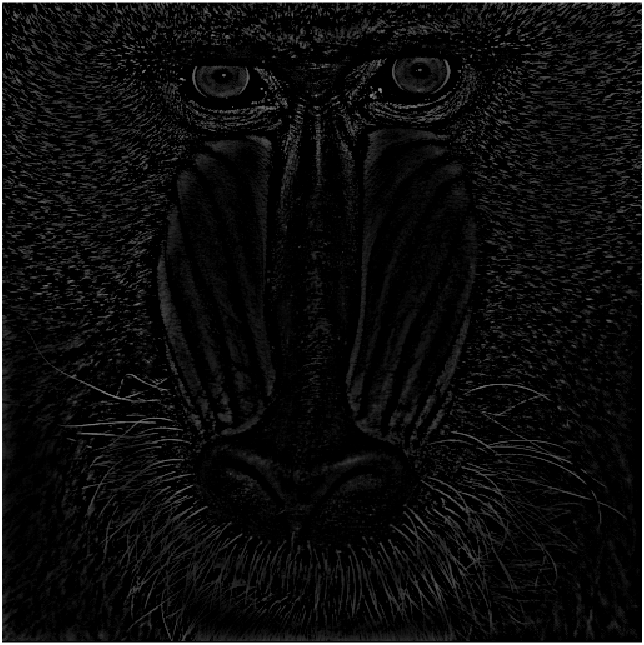
\includegraphics[width=0.8\linewidth]{Baboon_detail.png}
		\caption{Baboon detail}
	\end{minipage}
	\begin{minipage}{0.49\linewidth}
		\centering
		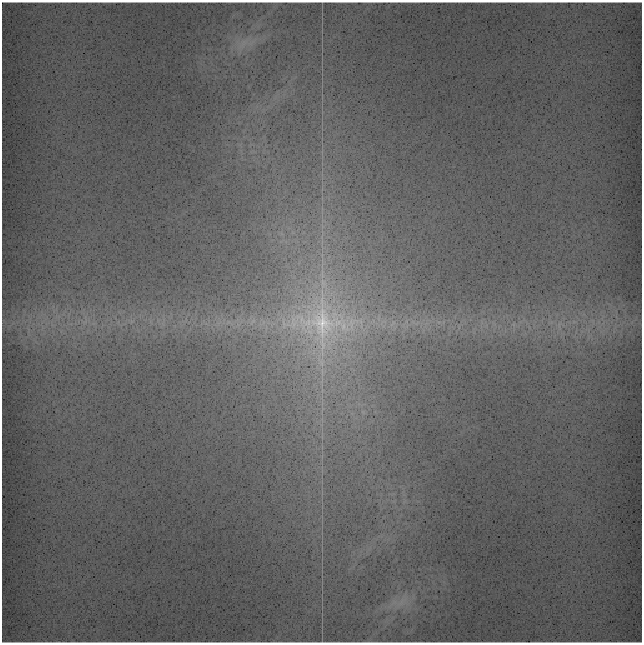
\includegraphics[width=0.8\linewidth]{Goldhill_freq.png}
		\caption{original frequency spectrum}
	\end{minipage}
\end{figure}


\item[(e)] Please design a notch filter to denoise 'Goldhill\_noised.tif'. The frequency spectrum of noiseless image is displayed above. Show the frequency spectrum of 'Goldhill\_noised.tif' and your denoised result. (12 pts)

\end{itemize}
\textbf{Solution:}
\begin{itemize}
	\item [(a)] The frequency spectrum is shown in Figure~\ref{fig:p1a}.
	\item [(b)] The image of filter of ideal and Butterworth filter and their processed image are shown in Figure~\ref{fig:ideal} and Figure~\ref{fig:BW} respectively.
	\item [(c)] The image processed by the ideal low-pass filter has the wave effect while the one processed by the Butterworth filter is more smooth.
				To explain this phenomenon, we can compare the spatial kernel of ideal and Butterworth low-pass filter (shown in Figure~\ref{fig:spatial_comparasion}).
				We can discover that the spatial kernel of ideal low-pass filter has serious wave effect and that's the reason why the processed image has serious wave effect.
	\item [(d)] I use a Gaussian High-pass filter with cut-out frequency $D_0=30$ to extract the detail of Baboon (set all value < 0 to 0 after processing) and the result is shown in Figure~\ref{fig:baboon_detail}.
	\item [(e)] After applying DFT to "Goldhill\_noised.tif", I discovered that its frequency spectrum has six obvious noisy patterns with very clear edges which shown in Figure~\ref{fig:noise_pattern},
				so I utilize ideal highpass filter to design the notch filter, the frequency spectrum after denoising is shown in Figure~\ref{fig:denoised_freq} and the denoised image is shown in Figure~\ref{fig:denoised_res}.		
\end{itemize}
\begin{figure}[H]
	\centering
	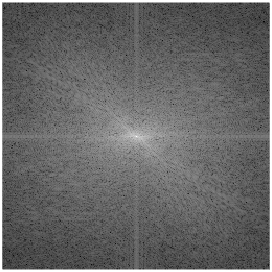
\includegraphics[width=0.2\textwidth]{images/p1a/frequency_spectrum.png}
	\caption{Frequency spectrum of Lena.tif}
	\label{fig:p1a}
	\subfigure[Image of ideal low-pass filter and its processed image]{
		
\includegraphics[width=0.2\textwidth]{images/p1b/ideal_filter.png}
		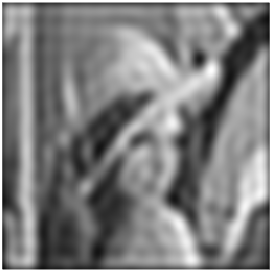
\includegraphics[width=0.2\textwidth]{images/p1b/ideal_res.png}
		\label{fig:ideal}
	}
	\subfigure[Image of Butterworth low-pass filter and its processed image]{
		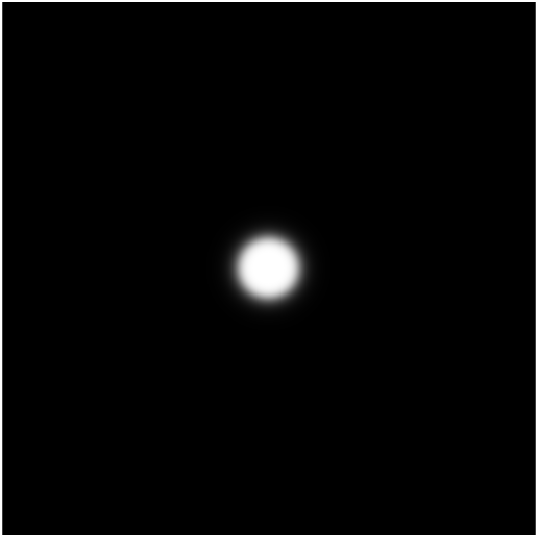
\includegraphics[width=0.2\textwidth]{images/p1b/BW_filter.png}
		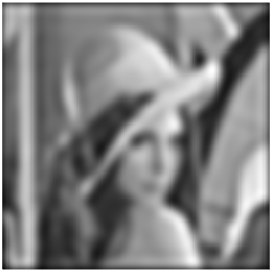
\includegraphics[width=0.2\textwidth]{images/p1b/BW_res.png}
		\label{fig:BW}
	}
	\caption{}
	
\includegraphics[width=0.3\textwidth]{images/p1b/ideal_spatial.png}
	
\includegraphics[width=0.3\textwidth]{images/p1b/BW_spatial.png}
	\caption{Comparasion between ideal and Butterworth filter in spatial domain}
	\label{fig:spatial_comparasion}
\end{figure}
	
\begin{figure}[H]
	\centering
	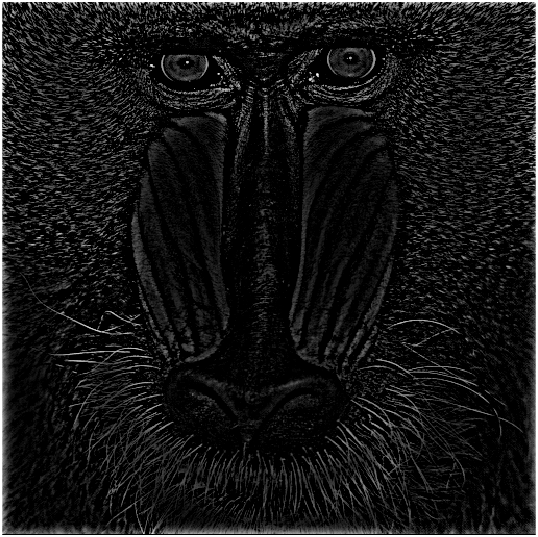
\includegraphics[width=0.3\textwidth]{images/p1d/detail.png}
	\caption{The extracted details of Baboon.tif}
	\label{fig:baboon_detail}
	\subfigure[Frequency spectrum of noise image]{
		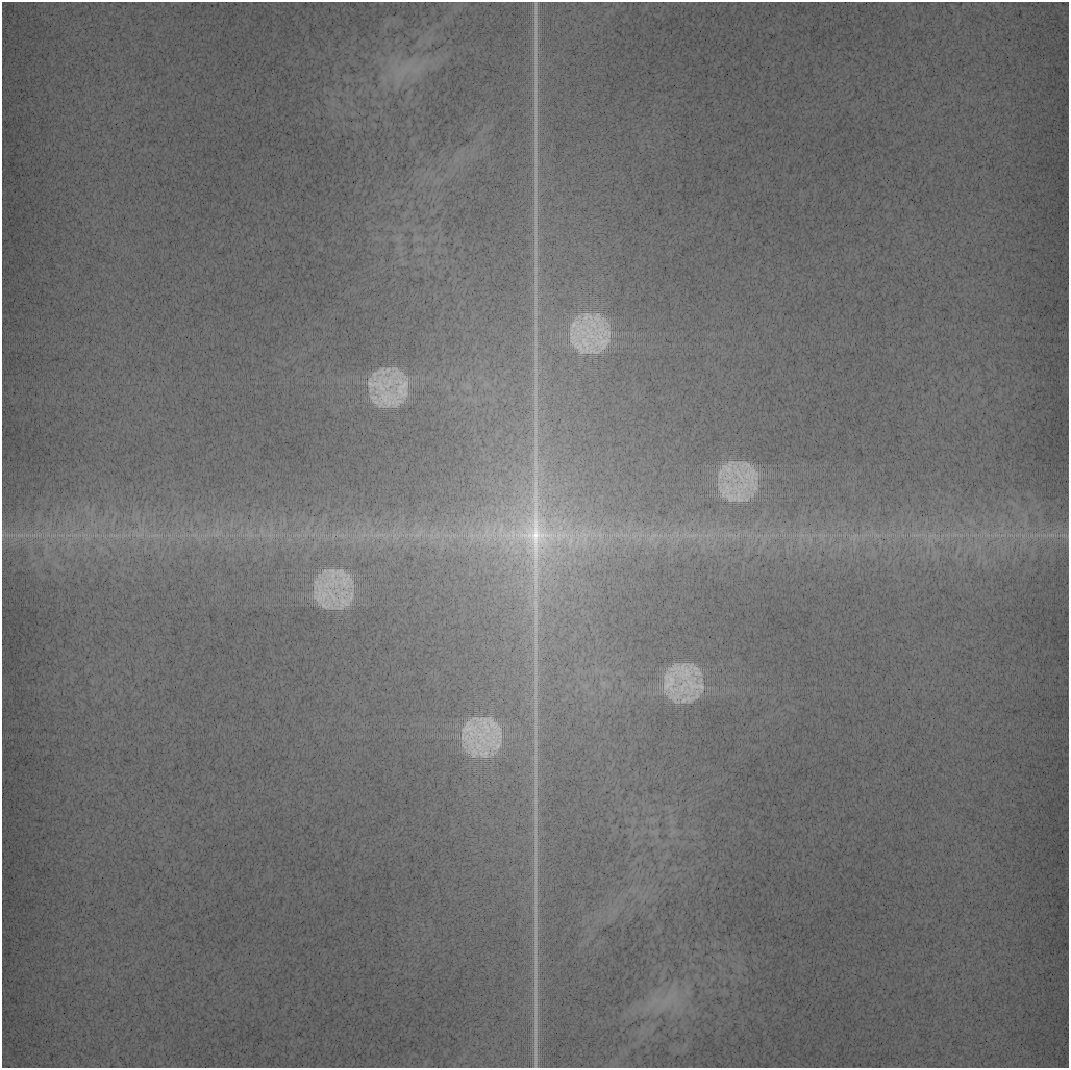
\includegraphics[width=0.25\textwidth]{images/p1e/noise_pattern.png}
		\label{fig:noise_pattern}
	}
	\subfigure[Frequency spectrum of denoised image]{
		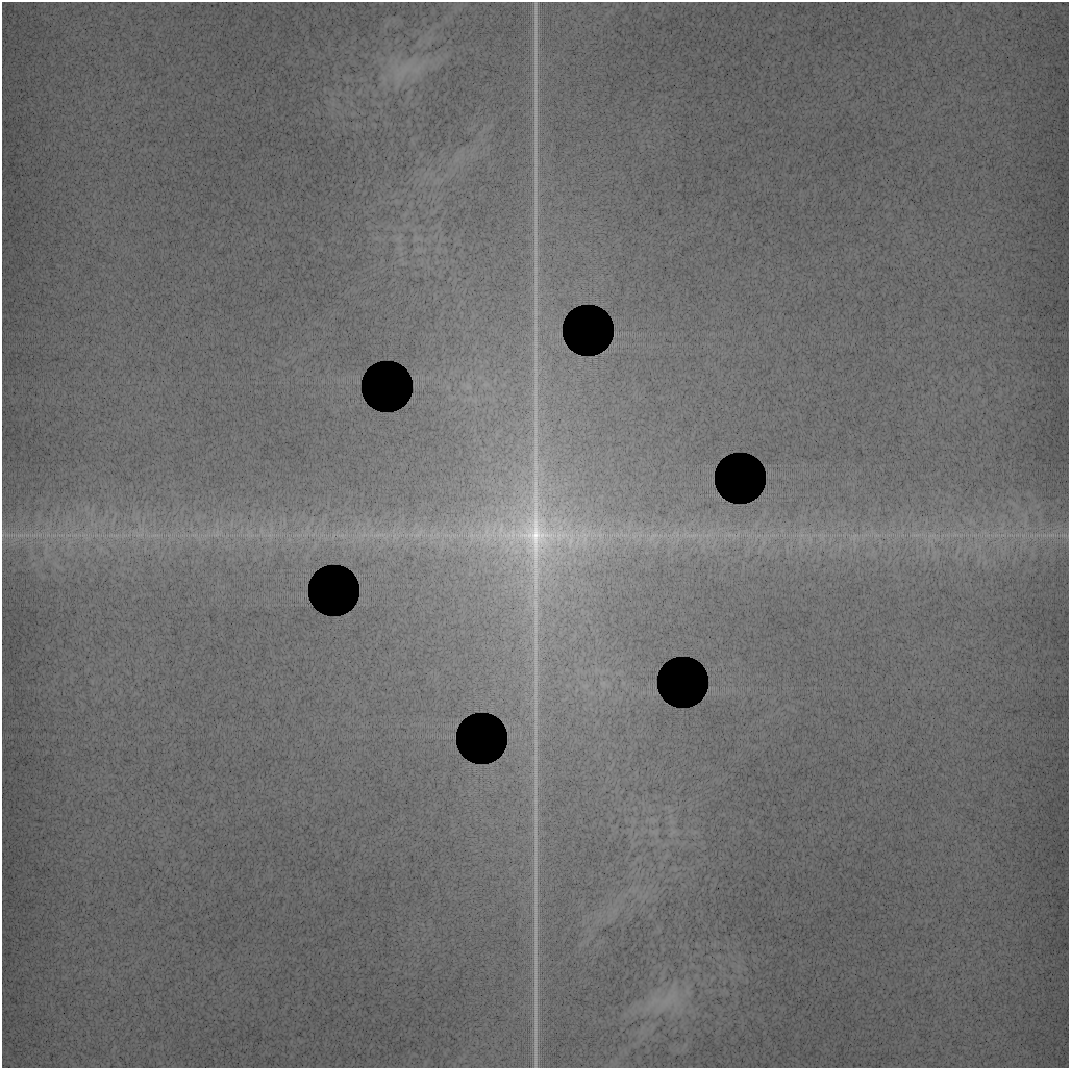
\includegraphics[width=0.25\textwidth]{images/p1e/denoised_freq.png}
		\label{fig:denoised_freq}
	}
	\subfigure[Denoised image]{
		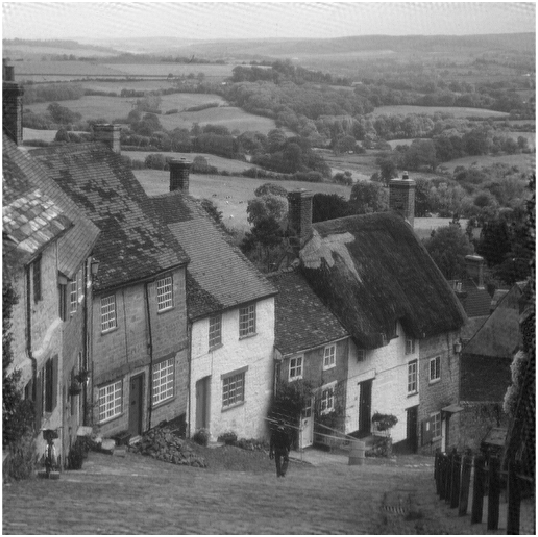
\includegraphics[width=0.25\textwidth]{images/p1e/denoised_res.png}
		\label{fig:denoised_res}
	}
	\caption{}
\end{figure}

\clearpage


\subsection*{Problem 2 (41 pts)}

\begin{itemize}
\item[(a)] Given a degraded image 'child\_degraded.tif' and the degradation function $H_1$. Restore the image with full inverse filter and inverse filter with proper cut-off, respectively. Show the results, and explain why full inverse filter works bad. (12 pts)
\item[(b)] Given a motion blur degradation function $H_2$, 
apply $H_2$ to 'child.tif' and show the blurred image. Try to restore the blurred image using inverse filter with proper cut-off. Explain why this restoration is more difficult than $H_1$  (restoration result doesn't need to show). (8 pts)



\item[(c)] Given a set of projection data, try to reconstruct the image using filtered back-projection with ramp filter, i.e. $|\omega|$. The reconstruction is like this:\\

\includegraphics[width=0.3\linewidth]{rec.png}\\
Show your filtered data and the reconstructed image (Hint: function 'imrotate', 'interp', and 'interp2' may be helpful in back-projection, but 'iradon' is not allowed). (15 pts)
\item[(d)] Apply hann window to ramp filter, then reconstruct the image again, show the image, describe the function of applying hann window in this question (Hint: hann window can be generated by function 'hann'). (6 pts)

\end{itemize}
\textbf{Solution:}
\begin{itemize}
	\item [(a)] The results of full inverse filter and cut-off inverse filter are shown in Figure~\ref{fig:full_cutoff}.
				The reason why the full inverse filter works badly is that there is an unknown noise term $N$ which affects the restoration tremendously.
				By definition, the DFT of the restored image has the form $\hat{F} = \frac{G}{H}+\frac{N}{H}$ where $G,H$ are the DFT of 
				the degraded image and the restoration function. Once $H$ contains $0$ or values vary close to $0$, then
				the term $\frac{N}{H}$ will goes to $\infty$ and become uncontrollable.
	\item [(b)] The blurred image is shown in Figure~\ref{fig:blur_res}. The reason why restoration by $H_2$ with cut-off 
				is more difficult than $H_1$ is that if we directly use $H_2$ to blur the image, the processed result contains
				no noise. In that case, applying an inverse filter with cut-off will lead to information loss.
	\item [(c)] The filtered data and the reconstructed image are shown in Figure~\ref{fig:p2c}.
	\item [(d)] The filtered data and the reconstructed image with hann window is shown in Figure~\ref{fig:p2d}. Applying hann window 
				helps to smooth the result. Similar to the case of ideal low-pass filter v.s. Butterworth filter, direct cutoff usually 
				introduce wave effect, we need a smooth window like hann window to eliminate the tremendous oscillation and get a smooth result.
\end{itemize}

\begin{figure}
	\centering
	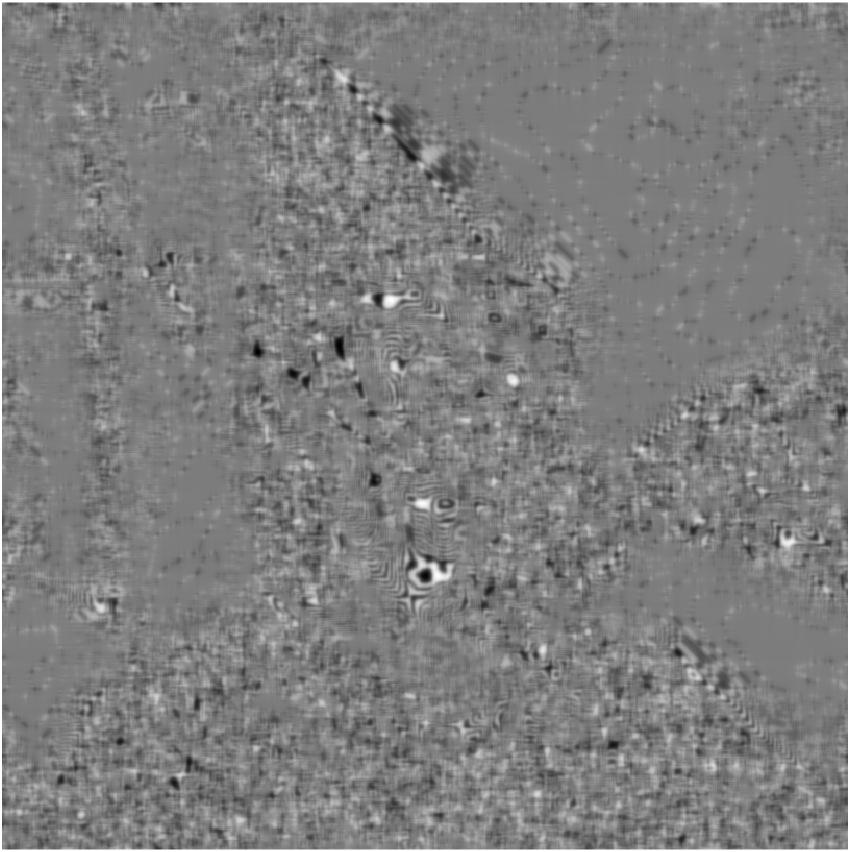
\includegraphics[width=0.25\textwidth]{images/p2a/full_res.png}
	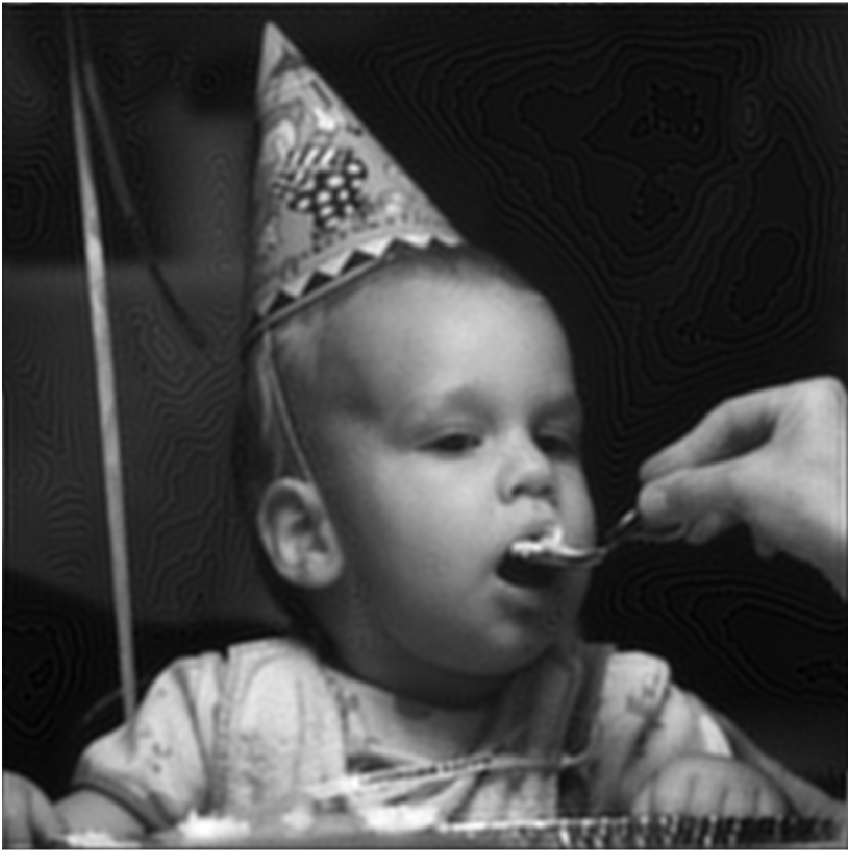
\includegraphics[width=0.25\textwidth]{images/p2a/cutoff_res.png}
	\caption{Results of full and cutoff inverse filter}
	\label{fig:full_cutoff}
	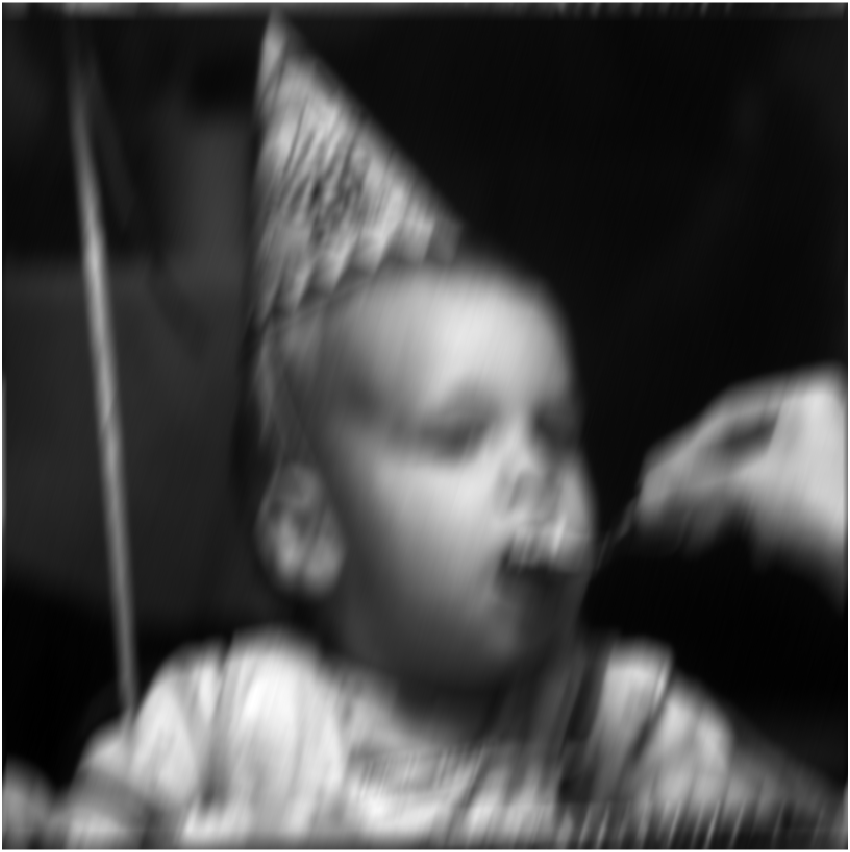
\includegraphics[width=0.25\textwidth]{images/p2b/blur_res.png}
	\caption{Blurred image}
	\label{fig:blur_res}
	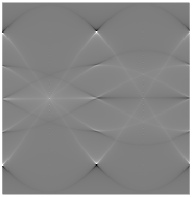
\includegraphics[width=0.25\textwidth]{images/p2c/filtered_data.png}
	
\includegraphics[width=0.25\textwidth]{images/p2c/restored_res.png}
	\caption{filtered data and reconstruction result}
	\label{fig:p2c}
	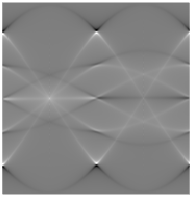
\includegraphics[width=0.25\textwidth]{images/p2d/han_data.png}
	
\includegraphics[width=0.25\textwidth]{images/p2d/han_res.png}
	\caption{filtered data and reconstruction result with hann window}
	\label{fig:p2d}
\end{figure}

\clearpage

\subsection*{Problem 3 (22 pts)}
\begin{itemize}
\item[(a)] Please convert 'PeppersRGB.tif' from RGB to HSI color space, and then convert it back. Show the image in HSI space and the recovered result in RGB space (Hint: you need to normalize all channels to [0, 1] in HSI space. Also, some exceptional values need to be judged individually). (16 pts)\\
Results are like this (displayed by imshow(img, [])):\\
\begin{figure}[htbp]
	\centering
	\begin{minipage}{0.49\linewidth}
		\centering
		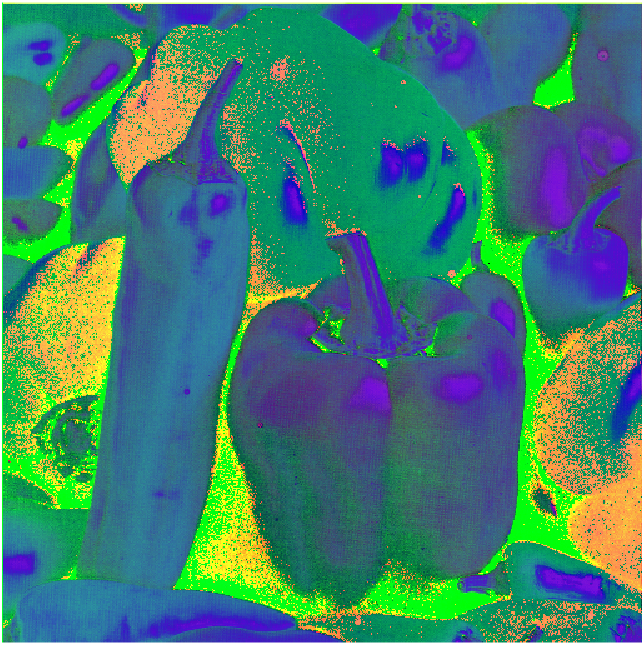
\includegraphics[width=0.8\linewidth]{hsi_space.png}
		\caption{HSI space}
	\end{minipage}
	\begin{minipage}{0.49\linewidth}
		\centering
		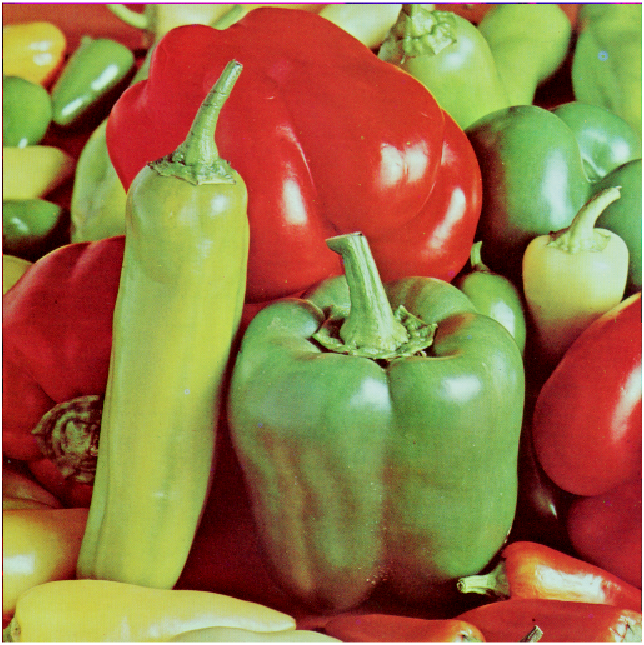
\includegraphics[width=0.8\linewidth]{rgb_space.png}
		\caption{RGB space}
	\end{minipage}
\end{figure}
\item[(b)] Choose proper structure element to conduct morphological operation to remove black points inside the object in 'guitar.tif' (6 pts)
\end{itemize}
\textbf{Solution:}
\begin{itemize}
	\item [(a)] The HSI space result and RGB space result are shown in Figure~\ref{fig:p3a}.
	\item [(b)] I chose first dilation and then erosion to eliminate the black points inside the object with $5\times 5$ structuring element (all ones).
				The result is shown in Figure~\ref{fig:p3b}.
\end{itemize}
\begin{figure}
	\centering
	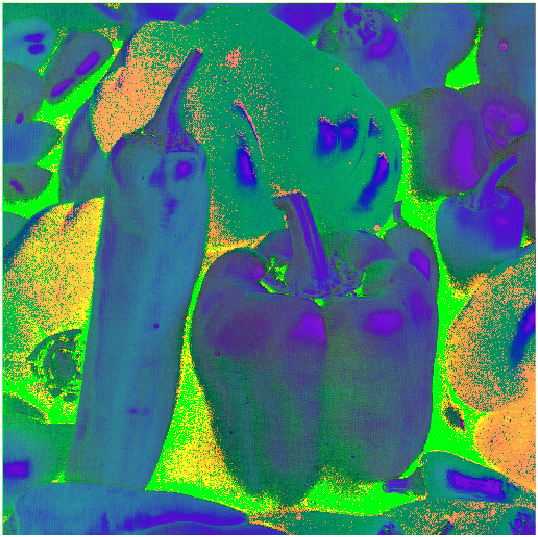
\includegraphics[width=0.25\textwidth]{images/p3a/HSI.png}
	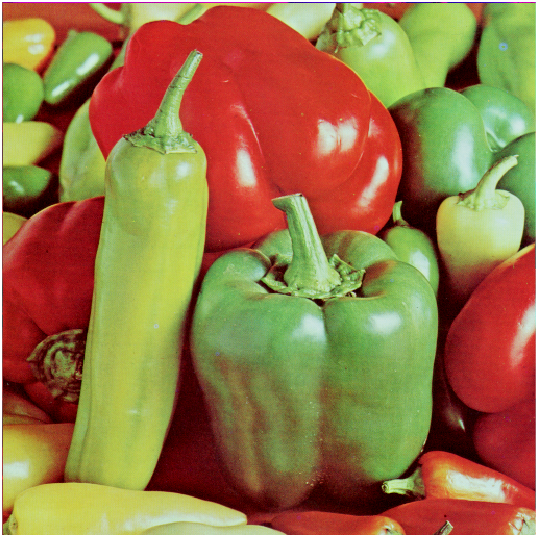
\includegraphics[width=0.25\textwidth]{images/p3a/RGB.png}
	\caption{HSI and RGB space}
	\label{fig:p3a}
	
\includegraphics[width=0.25\textwidth]{images/p3b/guitar_res.png}
	\caption{Result after dilation and erosion}
	\label{fig:p3b}
\end{figure}








\end{document}
https://www.overleaf.com/project/64171ae004389a062427825b